\chapter{ Analyse et Sp\'{e}cifications besoins }
\section{Introduction}


Cette partie consiste en une \'{e}tape analytique dans laquelle nous allons
recenser et factoriser les besoins des utilisateurs de l'application. Ceci est
fortement li\'{e} \`{a} l'\'{e}tude pr\'{e}alable men\'{e}e au
Cours du premier chapitre.
Pour ce faire cette phase doit r\'{e}pondre aux questions suivantes :
Quels sont les besoins fonctionnels de l'application ?
Quelles sont les contraintes qui doivent \^{e}tre prises en consid\'{e}ration?

   \section{ Les acteurs du syst\`{e}me }
C'est une entit\'{e} externe qui agit sur le syst\`{e}me (op\'{e}rateur, autre syst\`{e}me,
\ldots{}).Il peut consulter
Ou modifier l'\'{e}tat du syst\`{e}me.
En r\'{e}ponse \`{a} l'action d'un acteur, le syst\`{e}me fournit un service qui
correspond \`{a} son besoin.
Le principal acteur de syst\`{e}me :
\begin{itemize}
\item{  \textbf{L'administrateur :} entit\'{e} externe principale. Son r\^{o}le est qui a le droit de
g\'{e}rer un projet (cr\'{e}er, modifier, supprimer).
Aussi son r\^{o}le et de g\'{e}rer l'affectation des taches aux membres
correspondants.
}

\item{ \textbf{Le membre : } entit\'{e} externe secondaire, il peut se connecter pour consulter la
t\^{a}che en cours que l'administrateur lui a effectu\'{e} et la marquer comme
termin\'{e}e ou non.
}
\end{itemize}


\section{ Sp\'{e}cifications besoins}

  \subsection{Besoins fonctionnels}

Le besoin primordiale de notre application et de permettre à l’administrateur
de « Cherchini » de gérer les projets et ceci consiste à :

\subsubsection{G\'{e}rer les projets}

\begin{itemize}
\item{La cr\'{e}ation d’un projet.}
\item{La modification d'un projet.}
\item{La suppression d'un projet.}
\item{Consulter les projets et les t\^{a}che et les d\'{e}tails correspondants.}
\item{Affecter les membres correspondants \`{a} chaque projet.}
\end{itemize}

\subsubsection{G\'{e}rer les t\^{a}che}

\begin{itemize}
\item{La cr\'{e}ation d'une t\^{a}che.}
\item{La modification d'une t\^{a}che.}
\item{La suppression d'une t\^{a}che.}
\item{Consulter les t\^{a}che et les d\'{e}tails correspondants.}
\item{Affecter le membre correspondant \`{a} chaque t\^{a}che.}
\end{itemize}

\subsubsection{G\'{e}rer les membres}

\begin{itemize}
\item{La cr\'{e}ation d'un membre.}
\item{La modification d'un membre.}
\item{La suppression d'un membre.}
\item{Consulter les membres et leurs d\'{e}tails correspondants.}
\item{Affecter les membres correspondants \`{a} chaque projet.}
\end{itemize}

\subsubsection{G\'{e}rer les clients}

\begin{itemize}
\item{La cr\'{e}ation d'un .}
\item{La modification d'un client.}
\item{La suppression d'un client.}
\item{Consulter les clients et leurs d\'{e}tails correspondants.}
\end{itemize}

\subsubsection{
Suivre le d\'{e}roulement des projets}

\begin{itemize}
\item{ Suivre le travail des \'{e}quipes en consultant le diagramme Gantt pour chaque projet.}
\item{Consulter les rapports des co\^{u}ts et les dur\'{e}es selon les projets et les clients   .}
\item{Consulter la carte g\'{e}ographique des g\'{e}olocalisations des  .}
\end{itemize}

  \subsection{Besoins non fonctionnels}
Les besoins non fonctionnels sp\'{e}cifient les propri\'{e}t\'{e}s du syst\`{e}me afin de
garantir la Coh\'{e}rence, la confidentialit\'{e} et l'int\'{e}grit\'{e} des donn\'{e}es.
Le syst\`{e}me doit \^{e}tre fiable: la validit\'{e} de l`application.
R\'{e}utilisabilit\'{e}: aptitude de site \`{a} \^{e}tre utilis\'{e} en tout ou en partie dans de
nouvelles applications.

\subsubsection{La performance d'ex\'{e}cution}

Le temps d'ex\'{e}cution du syst\`{e}me doit \^{e}tre minimal pour ne pas g\^{e}ner
l'utilisateur. Ce temps d\'{e}pend de la complexit\'{e} du code impl\'{e}ment\'{e}, du
serveur d'application utilis\'{e}, du d\'{e}bit de la ligne de connexion et de la
conception de la base de donn\'{e}es.

\subsubsection{La s\'{e}curit\'{e}}

Le syst\`{e}me doit respecter un niveau de s\'{e}curit\'{e} \'{e}lev\'{e} afin de garantir la
confidentialit\'{e} de l'acc\`{e}s des membres

\subsubsection{L'ergonomie }

L'interface de cette application doit \^{e}tre ergonome, conviviale et voire m\^{e}me
apte \`{a} aider l'utilisateur \`{a} mieux g\'{e}rer son espace de travail.






\section{ Diagramme de cas d'utilisation g\'{e}n\'{e}rale }
Le diagramme de cas d'utilisation permet de d\'{e}crire l'interaction entre
l'acteur et le syst\`{e}me.
Le cas d'utilisation est une description des interactions qui vont permettre \`{a}
l'acteur d'atteindre son objectif en utilisant le syst\`{e}me. Un acteur et un cas
d'utilisation sont mis en relation par une association repr\'{e}sent\'{e}e par une
ligne.
Le but principal du diagramme du cas d'utilisation est de d\'{e}finir le syst\`{e}me
du point de vue des utilisateurs et de d\'{e}finir les limites pr\'{e}cises du syst\`{e}me en
utilisant une notation tr\`{e}s simple






\FloatBarrier
\begin{figure}[H]
\center
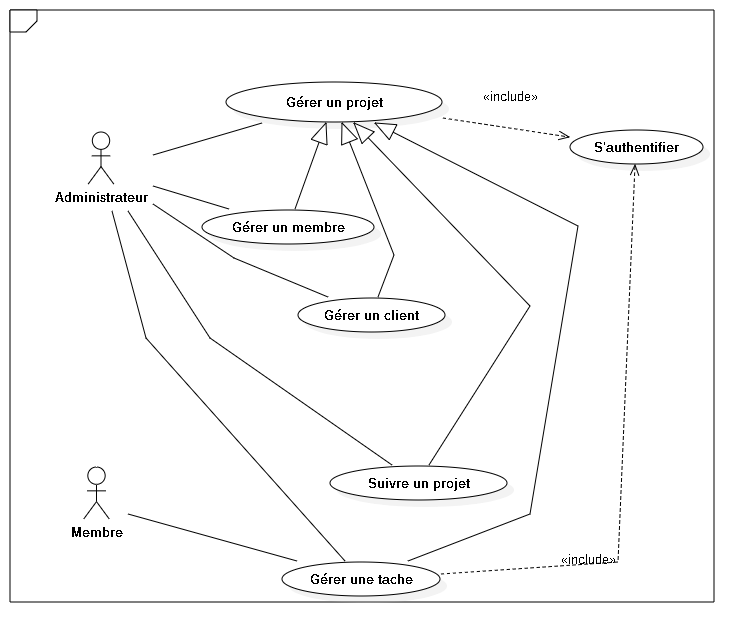
\includegraphics[width=13cm,height=10cm]{./figures/ucG.png}
\caption{Diagramme de cas d'utilisation g\'{e}n\'{e}rale.}

\end{figure}
\FloatBarrier







%\begin{figure}[!h]
%\center
%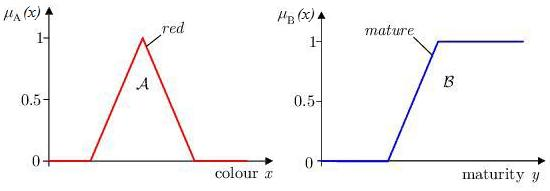
\includegraphics[width=10cm,height=6cm]{Relation.png}
%\caption{Titre de la Figure.}
%
%\end{figure}

%~~~~Bla bla bla exempe d'une liste:
%\begin{itemize}
%\item{}
%\item{}
%\item{}
%\item{}
%\end{itemize}

